\documentclass[12pt]{article}    
\usepackage{ucs} 
\usepackage[utf8x]{inputenc}
\usepackage[russian]{babel}  
\title{Лабораторная работа №2\\Машина Атвуда}
\author{Хафизов Фанис}
\usepackage[pdftex]{graphicx}

\begin{document}
	\begin{figure}
		\centering
		
\includegraphics[width=0.3\linewidth]{logo}
	\end{figure}
	\maketitle
	\newpage
	\section{Цель работы}
	Целью данной лабораторной работы является экспериментальное изучение закона равноускоренного движения связанных грузов на блоке и трактовка полученных результатов на основе рассмотрения динамики системы.
	\section{Схема установки}
	\begin{figure}[h]
		\centering
		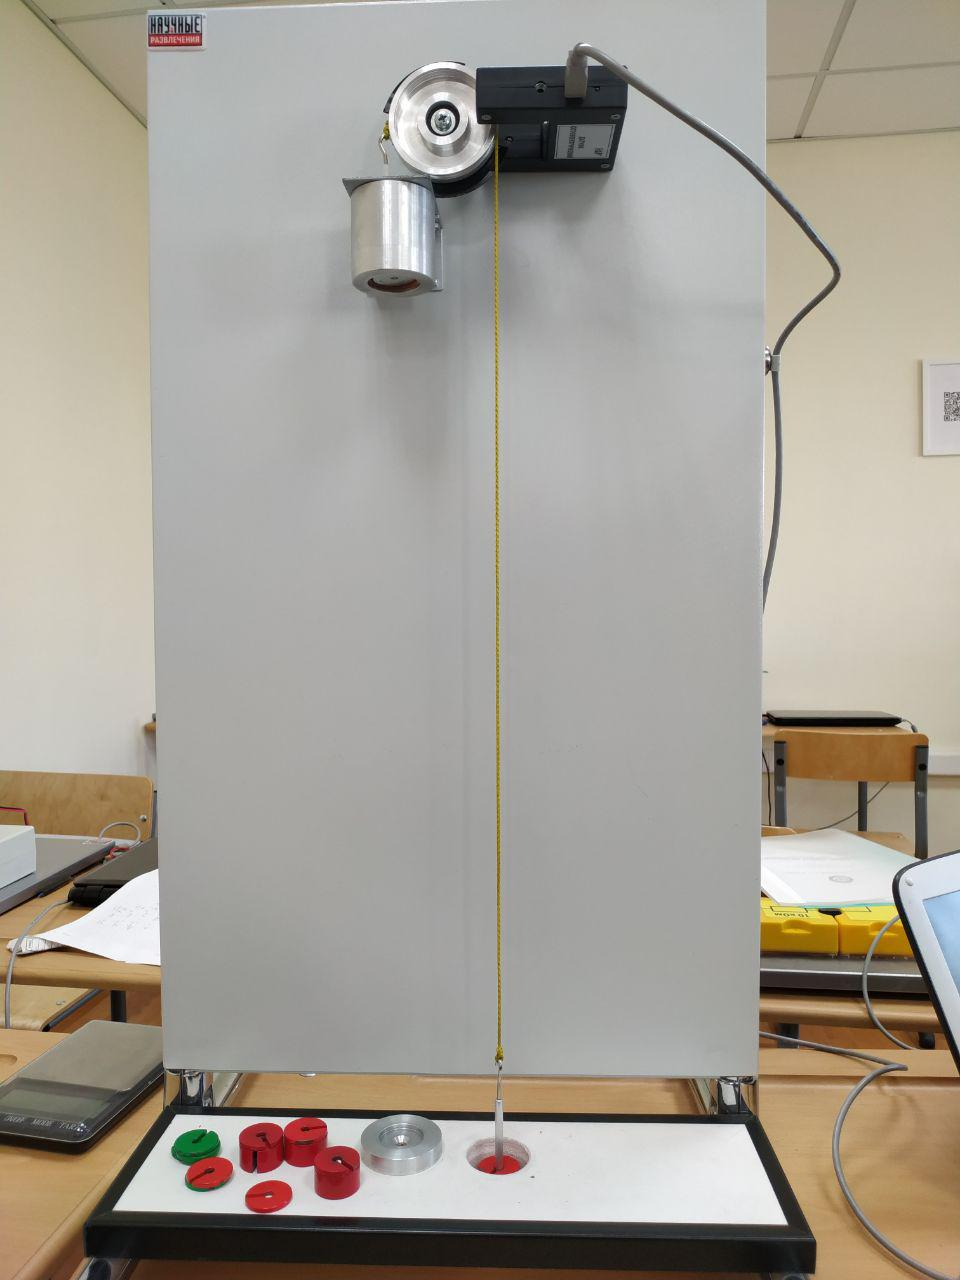
\includegraphics[width=0.3\linewidth]{scheme}
	\end{figure}
	Машина Атвуда представляет собой установку, на которой два
	одинаковых тяжелых груза массой m каждый, связаны нитью,
	перекинутой через блок.
	\section{Порядок действий}
	1)Соберем экспериментальную ускановку с суммарной массой грузов $M_1=170$ г и откроем программу на комьютере.\\
	2)Оттянем левый конец нити вниз, запустим измерения в программе. Построим в программе график зависимости $S(t)$, предварительно указав диаметр блока 60 мм.\\
	3)Переложим одну гирьку с левого груза на правый и повторим п. 2.
	Повторим эксперимент 4 раза и затем изменим суммарную массу гирек $M_2=70$ г.\\
	4)Построим график зависимости $a(dM)$.
	\section{Таблицы данных и графики}
	\begin{table}[h]
	\begin{tabular}{|l|l|l|l|l|}
		\hline
		& dM, кг & A     & B     & a, м/с$^2$ \\ \hline
		1 & 0,01   & 0,131 & 0,059 & 0,262      \\ \hline
		2 & 0,03   & 0,527 & 0,153 & 1,054      \\ \hline
		3 & 0,05   & 0,951 & 0,195 & 1,902      \\ \hline
		4 & 0,07   & 1,340 & 0,499 & 2,680      \\ \hline
	\end{tabular}
	\caption{a(dM)}
	\end{table}
	\begin{figure}[h]
		\centering
		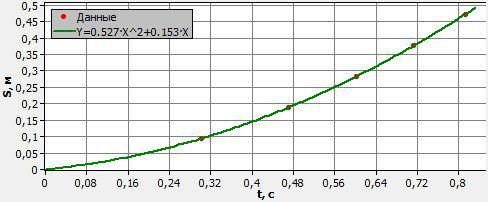
\includegraphics[scale=1.2]{graph1}
		\caption{График S(t)}
	\end{figure}
	\begin{figure}[h!]
		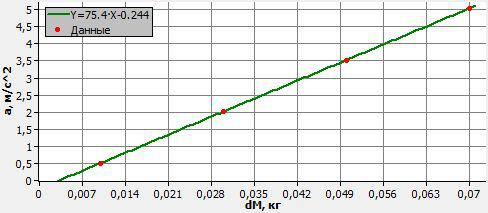
\includegraphics[scale=1.2]{graph2}
		\caption{График a(dM) для массы грузов $M_1$}
	\end{figure}
	\begin{figure}[h!]
		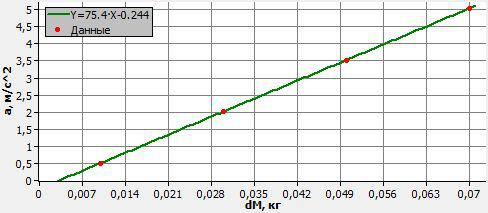
\includegraphics[scale=1.2]{graph3}
		\caption{График a(dM) для массы грузов $M_2$}
	\end{figure}
	\newpage
	\section{Расчеты}
	$k_1=40{,}5$ c$^{-2}$\\
	$k_2=75{,}4$ c$^{-2}$\\
	$g=\frac{k_1k_2(M_1-M_2)}{k_2-k_1}=\frac{40,5\cdot75,4(0,17-0,07)}{75,4-40,5}=8{,}750$ м/с$^2$\\
	$J_p=r^2(\frac{k_2(M_1-M_2)}{k_2-k_1}-M_1)=0,06^2(\frac{75,4*(0,17-0,07)}{75,4-40,5}-0{,}17)=0{,}000166$ кг$\cdot$м$^2$\\
	$J_{th}=\frac{1}{2}m_br^2=\frac{1}{2}0{,}055\cdot0{,}06^2=0{,}000099$ кг$\cdot$м$^2$\\
	$\varepsilon_g=\varepsilon_{k1}+\varepsilon_{k2}+\frac{\Delta M_1+\Delta M_2}{M_1-M_2}+\frac{\varepsilon_{k1}\cdot k_1+\varepsilon_{k2}\cdot k_2}{k_2-k_1}=\varepsilon_{dM}+\varepsilon_{dM}+\frac{\Delta M_1+\Delta M_2}{M_1-M_2}+\frac{\varepsilon_{dM}\cdot k_1+\varepsilon_{dM}\cdot k_2}{k_2-k_1}=2\cdot\frac{\Delta dM}{dM}+\frac{\Delta M_1+\Delta M_2}{M_1-M_2}+\frac{\frac{\Delta dM}{dM}\cdot k_1+\frac{\Delta dM}{dM}\cdot k_2}{k_2-k_1}=2\cdot\frac{0,0001}{0,02}+\frac{0,0007+0,0009}{0,170-0,070}+\frac{\frac{0,0001}{0,02}\cdot40,5+\frac{0,0001}{0,02}\cdot75,4}{75,4-40,5}=0,042$\\
	$\Delta g=\varepsilon_g*g=0{,}042*8{,}750=0{,}3675$ м/с$^2$\\
	\section{Результаты}
	$g=(8{,}750\pm 0{,}3675)$ м/с$^2$\\
	\section{Вывод}
	Мы получили не особо точный результат, с относительной погрешностью $4{,}2\%$. Для увеличения точности эксперимента можно было бы уменьшить трение в оси блока, а также использовать более точные грузики.\\
	Также мы оценили момент инерции блока и получили небольшое расхождение в теоретическом и практическом значениях. Объяснить это можно тем, что есть трение межди веревкой и блоком. 
\end{document}